\documentclass[a4paper]{article}

\usepackage{fancyhdr}
\usepackage{graphicx}
\usepackage{listings}

\graphicspath{ {./outputs/} }

\pagestyle{fancy}
\fancyhf{}
\rhead{Asim Bera}
\lhead{Programming in C}
\rfoot{Page \thepage}

\begin{document}

\tableofcontents
\newpage


\section{Assignment 1}

% begin subsection

\subsection{Write a C program to perform input/output of all basic data types.}
\textbf{Code}

\lstinputlisting[language=C]{programs/A01_P01.c}

\textbf{Output}

\begin{figure}[h]
  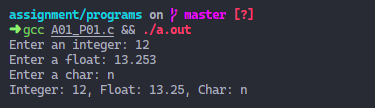
\includegraphics[width=12cm]{A01_P01.png}
\end{figure}

\newpage

% end subsection

% begin subsection

\subsection{Write a C program to enter two numbers and find their sum.}
\textbf{Code}

\lstinputlisting[language=C]{programs/A01_P02.c}

\textbf{Output}

\begin{figure}[h]
  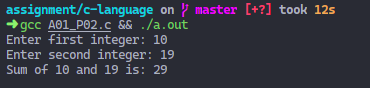
\includegraphics[width=12cm]{A01_P02}
\end{figure}

\newpage

% end subsection

% begin subsection

\subsection{Write a C program to enter two numbers and perform all arithmetic operations.}
\textbf{Code}

\lstinputlisting[language=C]{programs/A01_P03.c}

\textbf{Output}

\begin{figure}[h]
  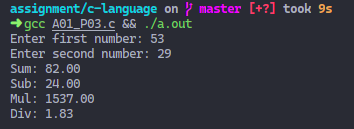
\includegraphics[width=12cm]{A01_P03}
\end{figure}

\newpage

% end subsection

% begin subsection

\subsection{Write a C program to enter length and breadth of a rectangle and find its perimeter.}
\textbf{Code}

\lstinputlisting[language=C]{programs/A01_P04.c}

\textbf{Output}

\begin{figure}[h]
  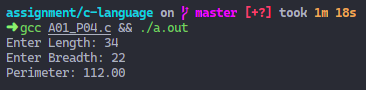
\includegraphics[width=12cm]{A01_P04}
\end{figure}

\newpage

% end subsection

% begin subsection

\subsection{Write a C program to enter length and breadth of a rectangle and find its area.}
\textbf{Code}

\lstinputlisting[language=C]{programs/A01_P05.c}

\textbf{Output}

\begin{figure}[h]
  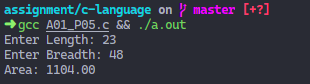
\includegraphics[width=12cm]{A01_P05}
\end{figure}

\newpage

% end subsection

% begin subsection

\subsection{Write a C program to enter radius of a circle find its diameter, circumference and area.}
\textbf{Code}

\lstinputlisting[language=C]{programs/A01_P06.c}

\textbf{Output}

\begin{figure}[h]
  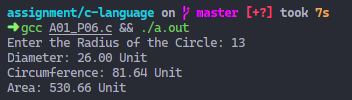
\includegraphics[width=12cm]{A01_P06}
\end{figure}

\newpage

% end subsection

% begin subsection

\subsection{Write a program to enter length in cm and convrt it into meter and kilometer.}
\textbf{Code}

\lstinputlisting[language=C]{programs/A01_P07.c}

\textbf{Output}

\begin{figure}[h]
  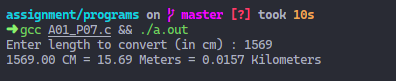
\includegraphics[width=12cm]{A01_P07}
\end{figure}

\newpage

% end subsection

% begin subsection

\subsection{Write a program to enter temperature in Celsius and convert it into Farenheit}
\textbf{Code}

\lstinputlisting[language=C]{programs/A01_P08.c}

\textbf{Output}

\begin{figure}[h]
  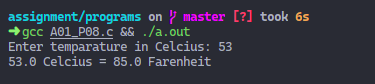
\includegraphics[width=12cm]{A01_P08}
\end{figure}

\newpage

% end subsection

% begin subsection

\subsection{Write a program to enter temperature in Farenheit and convert it into Celsius}
\textbf{Code}

\lstinputlisting[language=C]{programs/A01_P09.c}

\textbf{Output}

\begin{figure}[h]
  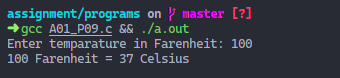
\includegraphics[width=12cm]{A01_P09}
\end{figure}

\newpage

% end subsection

% begin subsection

\subsection{Write a C program to convert days into years, weeks and days.}
\textbf{Code}

\lstinputlisting[language=C]{programs/A01_P10.c}

\textbf{Output}

\begin{figure}[h]
  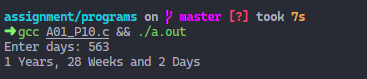
\includegraphics[width=12cm]{A01_P10}
\end{figure}

\newpage

% end subsection

% begin subsection

\subsection{Write a C program to find x\textsuperscript{y} of any number x and power y.}
\textbf{Code}

\lstinputlisting[language=C]{programs/A01_P11.c}

\textbf{Output}

\begin{figure}[h]
  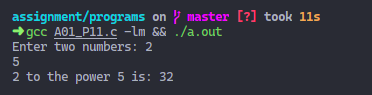
\includegraphics[width=12cm]{A01_P11}
\end{figure}

\newpage

% end subsection

% begin subsection

\subsection{Write a C program to enter any number and calculate its square root.}
\textbf{Code}

\lstinputlisting[language=C]{programs/A01_P12.c}

\textbf{Output}

\begin{figure}[h]
  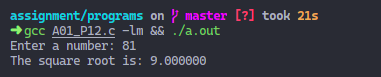
\includegraphics[width=12cm]{A01_P12}
\end{figure}

\newpage

% end subsection

% begin subsection

\subsection{Write a C program to enter two angles of a triangle and find its third angle.}
\textbf{Code}

\lstinputlisting[language=C]{programs/A01_P13.c}

\textbf{Output}

\begin{figure}[h]
  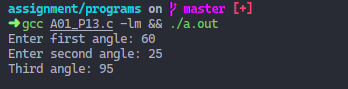
\includegraphics[width=12cm]{A01_P13}
\end{figure}

\newpage

% end subsection

% begin subsection

\subsection{Write a C program to enter base and height of a triangle and find its area.}
\textbf{Code}

\lstinputlisting[language=C]{programs/A01_P14.c}

\textbf{Output}

\begin{figure}[h]
  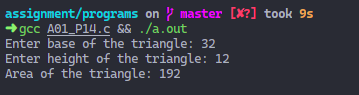
\includegraphics[width=12cm]{A01_P14}
\end{figure}

\newpage

% end subsection

% begin subsection

\subsection{Write a C program to calculate area of an equilateral triangle.}
\textbf{Code}

\lstinputlisting[language=C]{programs/A01_P15.c}

\textbf{Output}

\begin{figure}[h]
  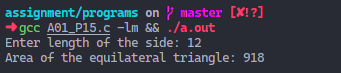
\includegraphics[width=12cm]{A01_P15}
\end{figure}

\newpage

% end subsection

% begin subsection

\subsection{Write a C program to enter marks of five subjects and calculate total, average and percentage.}
\textbf{Code}

\lstinputlisting[language=C]{programs/A01_P16.c}

\textbf{Output}

\begin{figure}[h]
  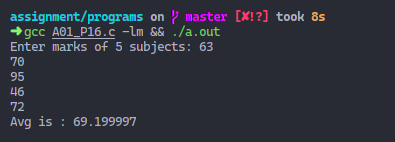
\includegraphics[width=12cm]{A01_P16}
\end{figure}

\newpage

% end subsection

% begin subsection

\subsection{Write a C program to enter P, T, R and calculate Simple Interest.}
\textbf{Code}

\lstinputlisting[language=C]{programs/A01_P17.c}

\textbf{Output}

\begin{figure}[h]
  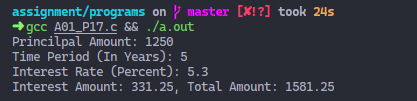
\includegraphics[width=12cm]{A01_P17}
\end{figure}

\newpage

% end subsection

% begin subsection

\subsection{Write a C program to enter P, T, R and calculate Compound Interest.}
\textbf{Code}

\lstinputlisting[language=C]{programs/A01_P18.c}

\textbf{Output}

\begin{figure}[h]
  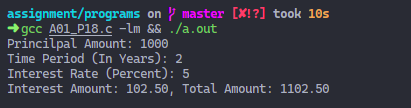
\includegraphics[width=12cm]{A01_P18}
\end{figure}

\newpage

% end subsection



\end{document}
